% Options for packages loaded elsewhere
\PassOptionsToPackage{unicode}{hyperref}
\PassOptionsToPackage{hyphens}{url}
\PassOptionsToPackage{dvipsnames,svgnames,x11names}{xcolor}
\documentclass[
  11pt,
]{article}
\usepackage{xcolor}
\usepackage[margin=1in]{geometry}
\usepackage{amsmath,amssymb}
\setcounter{secnumdepth}{-\maxdimen} % remove section numbering
\usepackage{iftex}
\ifPDFTeX
  \usepackage[T1]{fontenc}
  \usepackage[utf8]{inputenc}
  \usepackage{textcomp} % provide euro and other symbols
\else % if luatex or xetex
  \usepackage{unicode-math} % this also loads fontspec
  \defaultfontfeatures{Scale=MatchLowercase}
  \defaultfontfeatures[\rmfamily]{Ligatures=TeX,Scale=1}
\fi
\usepackage{lmodern}
\ifPDFTeX\else
  % xetex/luatex font selection
\fi
% Use upquote if available, for straight quotes in verbatim environments
\IfFileExists{upquote.sty}{\usepackage{upquote}}{}
\IfFileExists{microtype.sty}{% use microtype if available
  \usepackage[]{microtype}
  \UseMicrotypeSet[protrusion]{basicmath} % disable protrusion for tt fonts
}{}
\makeatletter
\@ifundefined{KOMAClassName}{% if non-KOMA class
  \IfFileExists{parskip.sty}{%
    \usepackage{parskip}
  }{% else
    \setlength{\parindent}{0pt}
    \setlength{\parskip}{6pt plus 2pt minus 1pt}}
}{% if KOMA class
  \KOMAoptions{parskip=half}}
\makeatother
\usepackage{longtable,booktabs,array}
\newcounter{none} % for unnumbered tables
\usepackage{calc} % for calculating minipage widths
% Correct order of tables after \paragraph or \subparagraph
\usepackage{etoolbox}
\makeatletter
\patchcmd\longtable{\par}{\if@noskipsec\mbox{}\fi\par}{}{}
\makeatother
% Allow footnotes in longtable head/foot
\IfFileExists{footnotehyper.sty}{\usepackage{footnotehyper}}{\usepackage{footnote}}
\makesavenoteenv{longtable}
\usepackage{graphicx}
\makeatletter
\newsavebox\pandoc@box
\newcommand*\pandocbounded[1]{% scales image to fit in text height/width
  \sbox\pandoc@box{#1}%
  \Gscale@div\@tempa{\textheight}{\dimexpr\ht\pandoc@box+\dp\pandoc@box\relax}%
  \Gscale@div\@tempb{\linewidth}{\wd\pandoc@box}%
  \ifdim\@tempb\p@<\@tempa\p@\let\@tempa\@tempb\fi% select the smaller of both
  \ifdim\@tempa\p@<\p@\scalebox{\@tempa}{\usebox\pandoc@box}%
  \else\usebox{\pandoc@box}%
  \fi%
}
% Set default figure placement to htbp
\def\fps@figure{htbp}
\makeatother
\setlength{\emergencystretch}{3em} % prevent overfull lines
\providecommand{\tightlist}{%
  \setlength{\itemsep}{0pt}\setlength{\parskip}{0pt}}
\usepackage{bookmark}
\IfFileExists{xurl.sty}{\usepackage{xurl}}{} % add URL line breaks if available
\urlstyle{same}
\hypersetup{
  colorlinks=true,
  linkcolor={black},
  filecolor={Maroon},
  citecolor={Blue},
  urlcolor={blue},
  pdfcreator={LaTeX via pandoc}}

\author{}
\date{}

\begin{document}

\section{A formally specified warning criterion for collapse in
recursive
systems}\label{a-formally-specified-warning-criterion-for-collapse-in-recursive-systems}

\textbf{David Mullett}

Independent Researcher

ORCID: 0009-0004-2543-1664

\textbf{Corresponding author:} David Mullett ·
\href{mailto:d@loopzero.org}{\nolinkurl{d@loopzero.org}}

\begin{center}\rule{0.5\linewidth}{0.5pt}\end{center}

\subsection{One-Sentence Summary}\label{one-sentence-summary}

A warning criterion defined around a minimal no-progress obstruction,
formalized in Lean to make the claim boundary explicit, motivates a
testable pre-collapse signature that survives fair warning-budget
benchmarking across public markets and recommender systems, while tested
standard comparator configurations did not recover accepted operating
points on canonical public benchmarks.

\begin{center}\rule{0.5\linewidth}{0.5pt}\end{center}

\subsection{Abstract}\label{abstract}

Recursive systems can enter collapse-like regimes before overt failure
becomes visible. In such regimes, amplification, endogenous recycling,
and contraction of accessible state trajectories reinforce one another
while local updates remain internally coherent. We define the warning
criterion around a minimal no-progress obstruction, formalized in Lean
to make the claim boundary explicit, and instantiate it using three
telemetry witnesses: gain (G), recursive persistence (p), and diversity
(δ). Under explicit assumptions, the obstruction motivates a testable
empirical prediction: pre-collapse regimes should exhibit rising
amplification, rising recursive persistence, and declining diversity.

We evaluate this prediction on three independent recursive domains. On
two public benchmarks - a markets event family and an offline
MovieLens-25M recursive recommender replay - comparators are evaluated
under a matched false-positive contract that compares detectors at the
same alert budget rather than at arbitrary thresholds. On the canonical
segmented markets benchmark, no tested fast or slow comparator
configuration achieved the locked equal-false-positive band {[}0.03,
0.07{]}; the nearest nontrivial comparator (AC1) remained materially
above band, while the numerically nearest slow configurations were
trivial-silent. On the canonical 50-step recommender benchmark, no
tested fast or slow comparator configuration was accepted across more
than one hundred tested settings; the result was preserved at adjacent
40- and 60-step horizon variants. Directional witness summaries were
fully aligned on the canonical recommender benchmark and on the
canonical late-window markets summary, with bounded weakening of the
diversity component in wider markets summary windows. We therefore
interpret the markets bridge as localized and late-window strongest
rather than uniformly invariant across wider summary windows. In a third
recursive domain - LLM training-loop collapse, Shumailov et al.~(2024) -
secondary analysis on the paper's published per-generation trajectories
shows the witness triad's directional pattern in both preservation
regimes; matched false-positive comparator evaluation in this domain is
deferred to follow-up work.

These results support a bounded claim: a formally specified recursive
obstruction defines an explicit bridge to a measurable pre-collapse
footprint that can be evaluated under a fair alert-budget contract, and
tested standard comparator configurations did not recover accepted
operating points on canonical public benchmarks. Collapse-like regimes,
on this view, become operationally testable under explicit bridge
assumptions.

\begin{center}\rule{0.5\linewidth}{0.5pt}\end{center}

\subsection{Main Text}\label{main-text}

\subsubsection{A formally specified obstruction for recursive
collapse}\label{a-formally-specified-obstruction-for-recursive-collapse}

Many systems of scientific and practical interest are recursive: present
state shapes future state, and locally valid updates can reinforce their
own continuation. Collapse, catastrophic shift, and resilience loss are
well-established phenomena in complex systems (Scheffer et al., 2001;
Holling, 1973). In such recursive systems, collapse need not begin as
overt breakdown. Related recursive-collapse behavior has recently been
demonstrated in generative-model training loops, where repeated training
on recursively generated data degrades model behavior (Shumailov et al.,
2024). Building on the established early-warning and critical slowing
down literature, which has developed variance growth, autocorrelation
shifts, and threshold excursions as observables for critical-transition
detection (Scheffer et al., 2009; Scheffer et al., 2012; Carpenter et
al., 2011; Dakos et al., 2012), this paper begins from a complementary
starting point: a formally specified structural obstruction
characterizing one specific failure mode within the broader
recursive-collapse landscape.

We formalize this as a no-progress obstruction for recursive feedback
systems, verified in Lean (de Moura \& Ullrich, 2021; The mathlib
Community, 2020). In that formal setting, one strictly worsening update
coupled to monotone tethers can generate a cycle in which local
continuation remains possible while meaningful progress is lost. The
empirical question is therefore not whether one can engineer a useful
detector from arbitrary signals. It is whether this formally specified
obstruction admits an explicit bridge, under stated assumptions, to a
measurable pre-collapse footprint in observed recursive systems.

The formal obstruction is intentionally elementary. The Lean development
is not presented as a deep result about real markets, recommender
systems, or any particular empirical substrate. The public Lean artifact
contains three deliberately elementary components: an abstract
no-progress obstruction over preorders, a measurement-map bridge, and a
schematic G,p,δ-style telemetry specialization. Thus Lean verifies the
structural ordered-measurement obstruction and the schematic telemetry
specialization; it does not verify that real benchmark telemetry
supplies the required measurement map.

\subsubsection{Conditional telemetry
bridge}\label{conditional-telemetry-bridge}

The formal result does not itself specify a unique empirical measurement
scheme for collapse. Cascading failure in interdependent systems
provides structural motivation for treating recursive no-progress as a
distinct failure mode (Buldyrev et al., 2010). The formal result
identifies a class of recursive no-progress regimes in which local
continuation remains possible while meaningful forward improvement
becomes inaccessible. We therefore treat the bridge as conditional
rather than automatic: to relate the obstruction to data, we consider
recursive systems in which future updates depend partly on recent
internal outputs, partly on external input, and partly on the diversity
of accessible next states. Under this interpretation, collapse need not
first appear as abrupt breakdown. It may instead emerge as an observable
pre-collapse regime in which perturbations are increasingly amplified,
recent internally generated states increasingly determine subsequent
states, and the accessible state space contracts.

The empirical claim that real benchmark telemetry supplies such a
measurement map remains external to Lean. It is tested by the benchmark
protocol: the observed G,p,δ witnesses must satisfy the prespecified
bridge criterion before externally defined collapse events under the
locked false-positive contract, while comparator families are evaluated
under the same alert budget.

The obstruction therefore motivates three testable observable tendencies
before externally defined collapse events: rising gain G, indicating
amplification rather than damping of perturbation; rising recursive
persistence p (operationalized in the bridge criterion as a
non-relaxation gate), indicating increasing persistence of internally
generated state; and declining diversity δ, indicating contraction of
the effective range of system trajectories (Walker et al., 2004; Gao et
al., 2016). We use G, p, and δ as empirical proxies for amplification,
recursive persistence, and state-space contraction. This bridge is
explicitly falsifiable: it would be weakened if benchmark-defined
collapse repeatedly occurred without prior elevation of G and p and
reduction of δ, or if matched-false-positive comparator configurations
repeatedly recovered accepted operating points without this triad.

\emph{Scope summary.} (i) Lean verifies the abstract no-progress
obstruction over preorders, the bridge lemma
\texttt{collapse\_via\_progresscycle\_public}, and a schematic telemetry
specialization. (ii) The conditional bridge assumes that real recursive
systems admit a measurement function μ into a preorder under which the
witness triad is observable with the intended directional structure.
(iii) The benchmarks test whether the witness pattern in fact precedes
externally defined event labels under the locked equal-false-positive
contract; this is an empirical question, not a verified one.

\subsubsection{Telemetry witnesses and matched-false-positive
benchmarking}\label{telemetry-witnesses-and-matched-false-positive-benchmarking}

The bridge criterion is operationalized through a triplet of witnesses.
G estimates short-horizon amplification of perturbation, p estimates
short-horizon recursive persistence of active state, and δ estimates the
effective breadth of observed system behavior across channels, modes, or
trajectories. The predicate is therefore designed to test the empirical
signature implied by the formal mechanism, not to restate the formal
obstruction in observational language.

In the current implementation, the three witnesses are not equally
directional in their operational role. G is evaluated as an
elevated-gain condition relative to recent background, and δ is
evaluated through a non-increase condition over the relevant lookback
window. The p witness is used most conservatively: it functions as a
non-relaxation gate consistent with monotone-tether semantics rather
than as a standalone directional effect-size claim. In the
public-markets adapter, p is constructed from a trailing recurrence
statistic over stress events defined using a fixed z-threshold of 1.5;
this threshold is part of the current adapter definition and should be
interpreted as such.

All empirical evaluation is conducted under a matched false-positive
contract. In heterogeneous systems, comparator families can appear
competitive simply by spending false alarms differently (Boettiger \&
Hastings, 2012a; Diks et al., 2019). We therefore compare detectors only
at the same alert budget, defined by a locked equal-false-positive
criterion rather than by arbitrary family-specific thresholds (Boettiger
\& Hastings, 2012b; Hanley \& McNeil, 1982). A configuration is accepted
only if its control-unit false-positive rate lies within the
prespecified interval FP ∈ {[}0.03, 0.07{]}.

The acceptance band was chosen prior to evaluation to reflect the
operational alert burden plausible for an operator monitoring a
comparator unit population over a comparable observation period. A mean
false-positive rate of 0.05 corresponds to approximately one false alert
per 20 control-period units; the half-width of ±0.02 reflects acceptable
sampling variation under finite-control evaluation. Tighter bands such
as {[}0.01, 0.05{]} would be operationally desirable but require larger
control-unit populations than the canonical markets benchmark provides;
wider bands such as {[}0.05, 0.10{]} would inflate the false-alarm
budget beyond what is operationally tolerable in a deployed warning
context. The band was locked at this specification before any comparator
evaluation. We note that on the canonical markets benchmark with n=38
controls, the grid step 1/38 = 0.026316 admits only 2/38 control alarms
within the band (FP = 0.052632), making the band effectively a
single-grid-point target on that benchmark; the recommender benchmark
with n=4,755 controls (grid step 1/4755 = 0.0002103) is therefore the
empirically dispositive case, and the markets non-acceptance result
should be read as corroborating second-domain evidence rather than as an
independent statistical claim of comparator inadequacy.

Under this contract, the empirical program is directly falsifiable: it
fails if any comparator configuration admits an accepted operating point
on the canonical benchmark under the same criterion.

\subsubsection{Cross-domain evidence for a pre-collapse
signature}\label{cross-domain-evidence-for-a-pre-collapse-signature}

We therefore test whether the witness triad (G, p, δ) appears before
externally defined collapse events under a locked equal-false-positive
benchmark across heterogeneous recursive systems. Across retained domain
families, the criterion identifies pre-collapse structure before
externally defined breakdown or intervention points and does so under
the same alert-budget rule. These retained families were chosen not
because they are easy cases, but because they admit externally defined
event times, nontrivial controls, and fair comparator evaluation under a
common false-positive contract.

Directional witness summaries were fully aligned on the canonical
recommender benchmark. On the canonical public-markets benchmark, the
same directional pattern was recovered when markets were summarized over
the last 30 minutes of each exact canonical unit using G, p, and
diversity-change within the late window. In a wider 60-minute markets
summary, G and p remained directionally aligned whereas diversity-change
weakened. We therefore interpret the markets bridge as localized and
late-window strongest rather than uniformly invariant across wider
summary windows.

The broader significance is not that a new warning statistic works in
one domain. It is that a formally specified recursive obstruction
appears to support a domain-resolved empirical signature across systems
that differ strongly in substrate, timescale, and external semantics.
The evidence therefore supports an explicitly bounded empirical program
rather than a single-domain detector construction.

A domain-resolved witness-direction summary is provided in the
Supplementary Materials. The combined comparator calibration summary
across both flagship benchmarks is reported in Table 1.

\textbf{Table 1. Comparator calibration on the canonical public
benchmarks under the locked equal-false-positive contract (FP ∈ {[}0.03,
0.07{]}).}

{\def\LTcaptype{none} % do not increment counter
\begin{longtable}[]{@{}
  >{\raggedright\arraybackslash}p{(\linewidth - 12\tabcolsep) * \real{0.1429}}
  >{\raggedright\arraybackslash}p{(\linewidth - 12\tabcolsep) * \real{0.1429}}
  >{\raggedright\arraybackslash}p{(\linewidth - 12\tabcolsep) * \real{0.1429}}
  >{\raggedright\arraybackslash}p{(\linewidth - 12\tabcolsep) * \real{0.1429}}
  >{\raggedright\arraybackslash}p{(\linewidth - 12\tabcolsep) * \real{0.1429}}
  >{\raggedright\arraybackslash}p{(\linewidth - 12\tabcolsep) * \real{0.1429}}
  >{\raggedright\arraybackslash}p{(\linewidth - 12\tabcolsep) * \real{0.1429}}@{}}
\toprule\noalign{}
\begin{minipage}[b]{\linewidth}\raggedright
Benchmark
\end{minipage} & \begin{minipage}[b]{\linewidth}\raggedright
Comparator (family, role)
\end{minipage} & \begin{minipage}[b]{\linewidth}\raggedright
Configuration
\end{minipage} & \begin{minipage}[b]{\linewidth}\raggedright
Control FP
\end{minipage} & \begin{minipage}[b]{\linewidth}\raggedright
Event alarm rate
\end{minipage} & \begin{minipage}[b]{\linewidth}\raggedright
Distance from band
\end{minipage} & \begin{minipage}[b]{\linewidth}\raggedright
Status
\end{minipage} \\
\midrule\noalign{}
\endhead
\bottomrule\noalign{}
\endlastfoot
Markets (n=38 controls, 16 events) & AC1 (fast --- nearest nontrivial) &
\texttt{ac1\_ews\_\_632f23b2} & 0.1316 (5/38) & 0.0625 (1/16) & +0.0616
above & Above band \\
Markets & Permutation entropy (slow --- best nontrivial) &
\texttt{permutation\_entropy\_\_259c1b96} & 0.3684 (14/38) & 0.2500
(4/16) & +0.2984 above & Above band \\
Markets & Matrix profile / permutation entropy (slow --- numerically
nearest) & trivial-silent ties & 0.0000 (0/38) & 0.0000 (0/16) & --- &
Trivial-silent \\
Recommender (n=4,755 controls, 35,584 events; 105 configurations tested)
& Matrix profile (slow --- overall nearest) &
\texttt{matrix\_profile\_\_44b81bd6} & 0.01367 & 0.1107 & −0.0163 below
& Below band \\
Recommender & Variance EWS (fast --- nearest) & trivial-silent & 0.0000
& --- & --- & Trivial-silent \\
\end{longtable}
}

\emph{No tested comparator configuration achieved an accepted operating
point on either benchmark. Comparator calibration under the matched
false-positive contract is not equivalent to universal detector ranking;
comparators may admit competitive operating points under different
evaluation frameworks. The contract evaluates whether the prespecified
canonical band can be reached, not which detector is universally
superior.}

\subsubsection{Canonical public recommender
benchmark}\label{canonical-public-recommender-benchmark}

A second flagship benchmark was constructed from MovieLens-25M user
trajectories to test whether the bridge criterion survives outside
markets. Recommender systems are known to narrow accessible diversity
through feedback-driven filtering (Fleder \& Hosanagar, 2009). User
ratings were sorted chronologically, reduced to one episode per user,
and replayed under a deterministic item-item collaborative-filtering
engine with a warm-start prefix and a held-out positive frontier (Chaney
et al., 2018; Jiang et al., 2019; Mansoury et al., 2020). On the
canonical 50-step benchmark, 40,339 user-level units satisfied inclusion
criteria, including 35,584 event units and 4,755 control units. The
control-unit false-positive grid step was 1/4755 = 0.0002103, so the
prespecified acceptance band {[}0.03, 0.07{]} was reachable by
construction.

On this canonical recommender benchmark, the witness pattern satisfied
the prespecified bridge criterion in the pre-collapse window:
pre-collapse event units showed higher amplification G, higher recursive
persistence p, and lower diversity δ than reference controls. User-level
bootstrap summaries were directionally consistent with this pattern and
were used descriptively rather than as a significance test. Under the
same locked equal-false-positive contract, no tested fast or slow
comparator configuration admitted an accepted operating point. Across
105 tested configurations, the overall nearest comparator was matrix
profile (matrix\_profile\_\_44b81bd6), which remained below the lower
edge of the accepted band with control FP = 0.0136698, band distance =
0.0163302, and event alarm rate = 0.110668. Among fast families, the
numerically nearest operating point was a trivial-silent variance EWS
configuration at FP = 0.0, whereas the nearest nontrivial fast-family
configurations overfired controls substantially.

\pandocbounded{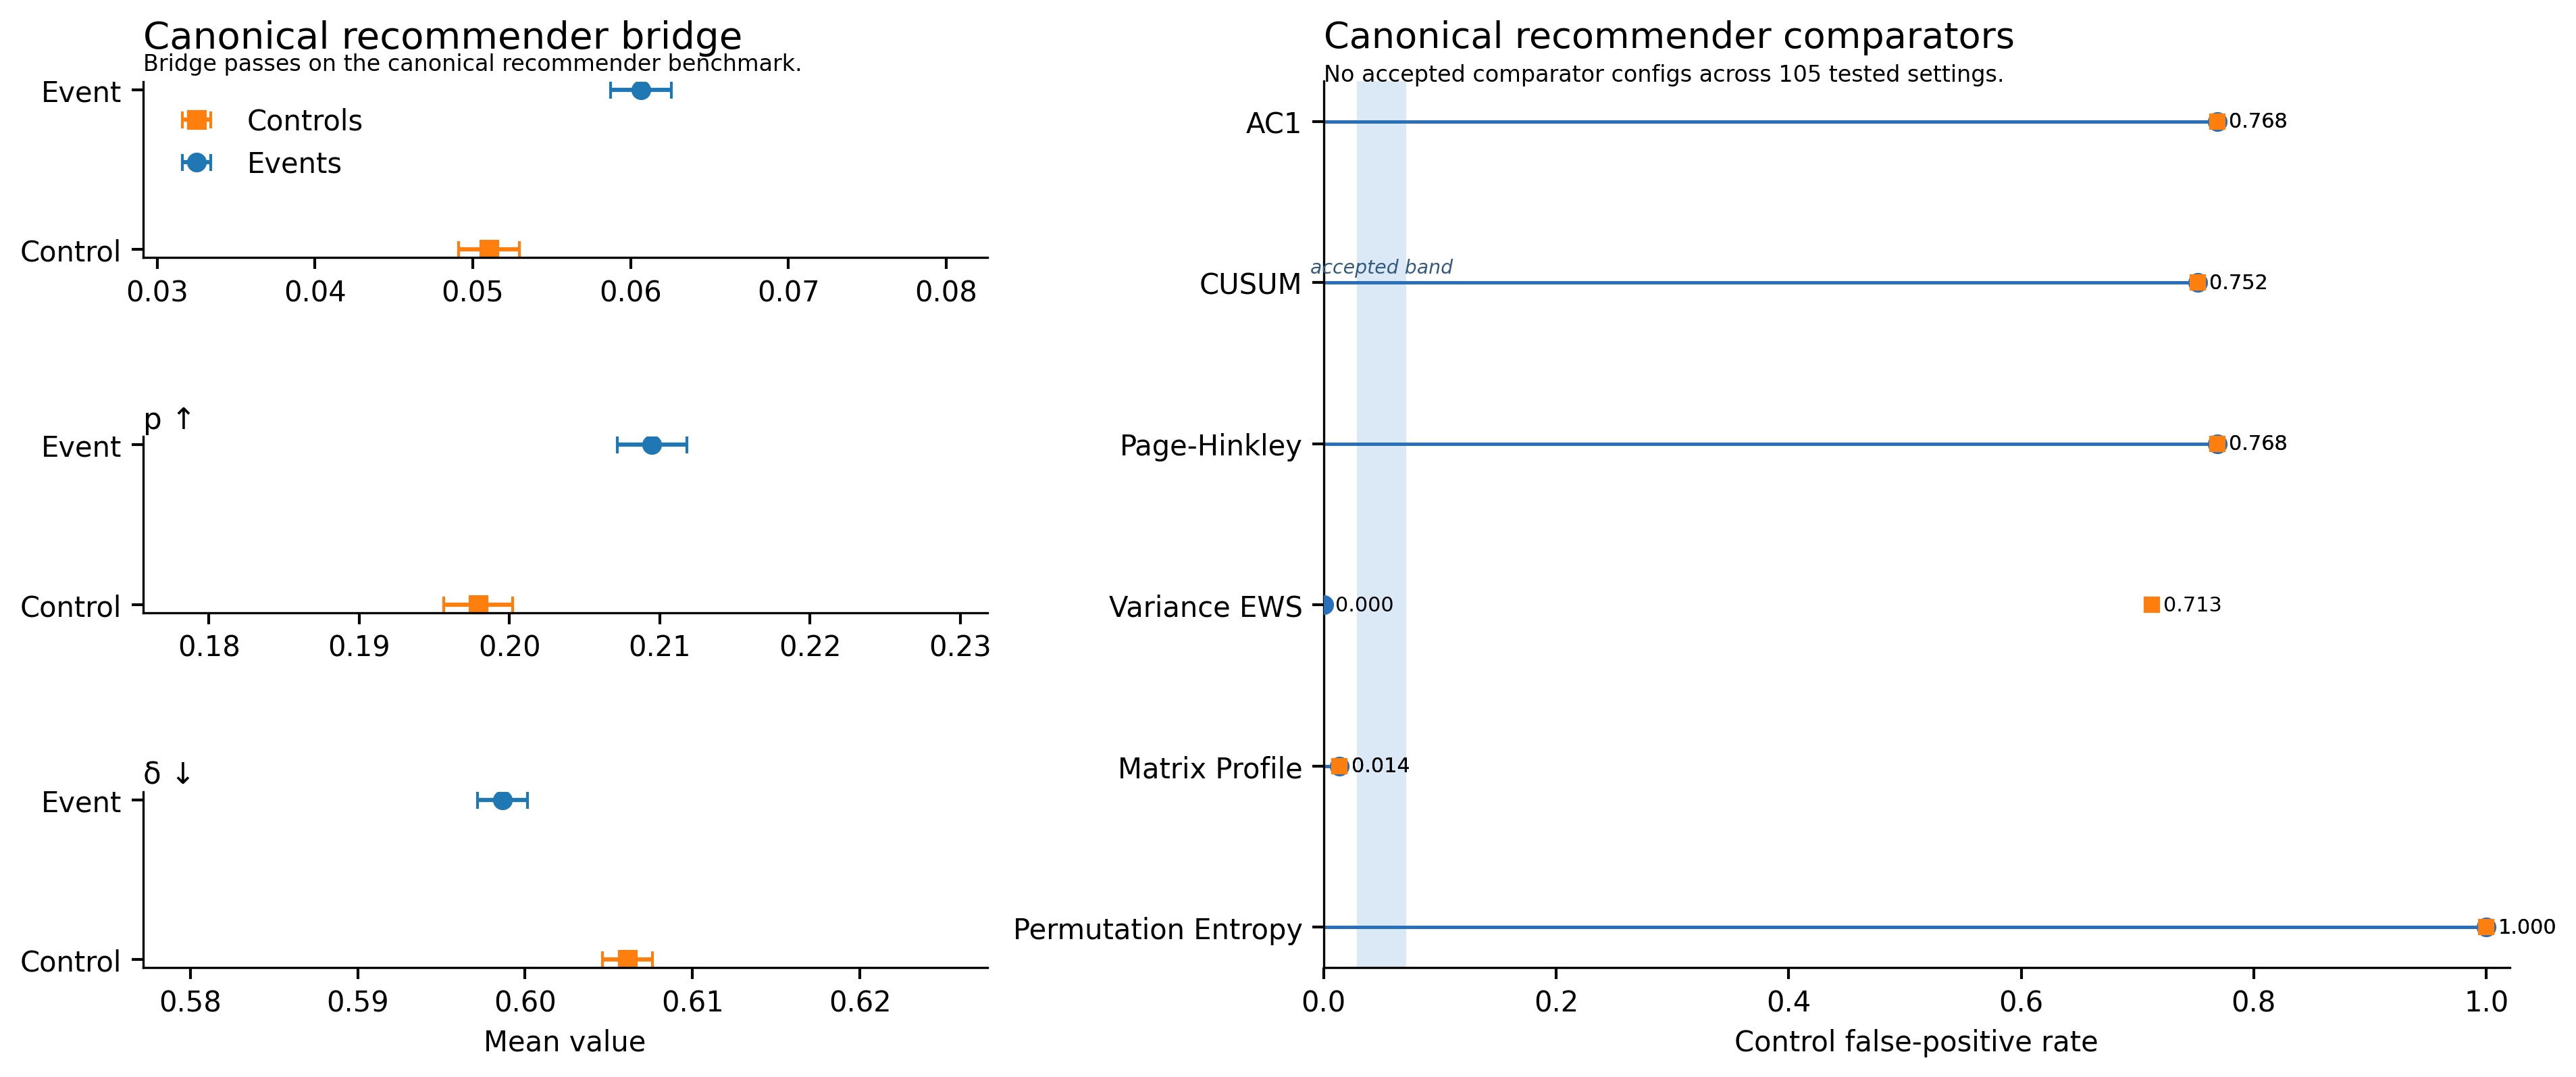
\includegraphics[keepaspectratio]{assets/fig2_recommender_canonical_bridge_and_comparators.png}}

\textbf{Figure 1. Canonical recommender benchmark: bridge summary and
comparator calibration.} On the canonical 50-step MovieLens benchmark,
directional witness summaries are fully aligned: event units show higher
gain G, higher recursive persistence p, and lower diversity δ than
controls. Under the same locked equal-false-positive contract, no tested
comparator configuration is accepted across 105 tested settings; the
overall nearest comparator is matrix profile at FP = 0.0136698, below
the lower edge of the accepted band. Results are based on offline
deterministic replay rather than deployed-system feedback.

\subsubsection{Recommender robustness under adjacent horizon
sensitivity}\label{recommender-robustness-under-adjacent-horizon-sensitivity}

To test whether the recommender result depended on the canonical episode
horizon, the benchmark was rebuilt at adjacent horizons of 40 and 60
recursive update steps while holding benchmark construction and
comparator rules fixed. At both adjacent horizons, no comparator
configuration recovered an accepted operating point under the locked
equal-false-positive band. The overall nearest comparator remained
matrix profile in all three horizon settings and remained outside the
accepted interval. The bridge criterion was satisfied at 60 steps but
only partially satisfied at 40 steps. This horizon dependence is
mechanistically expected: shorter pre-collapse windows leave less time
for the recursive signature to separate cleanly from matched controls.
The recommender branch therefore supports a corroborating second
flagship benchmark on the comparator claim, with a bounded robustness
qualification on the bridge layer under adjacent horizon shortening
rather than an unqualified invariance claim.

\pandocbounded{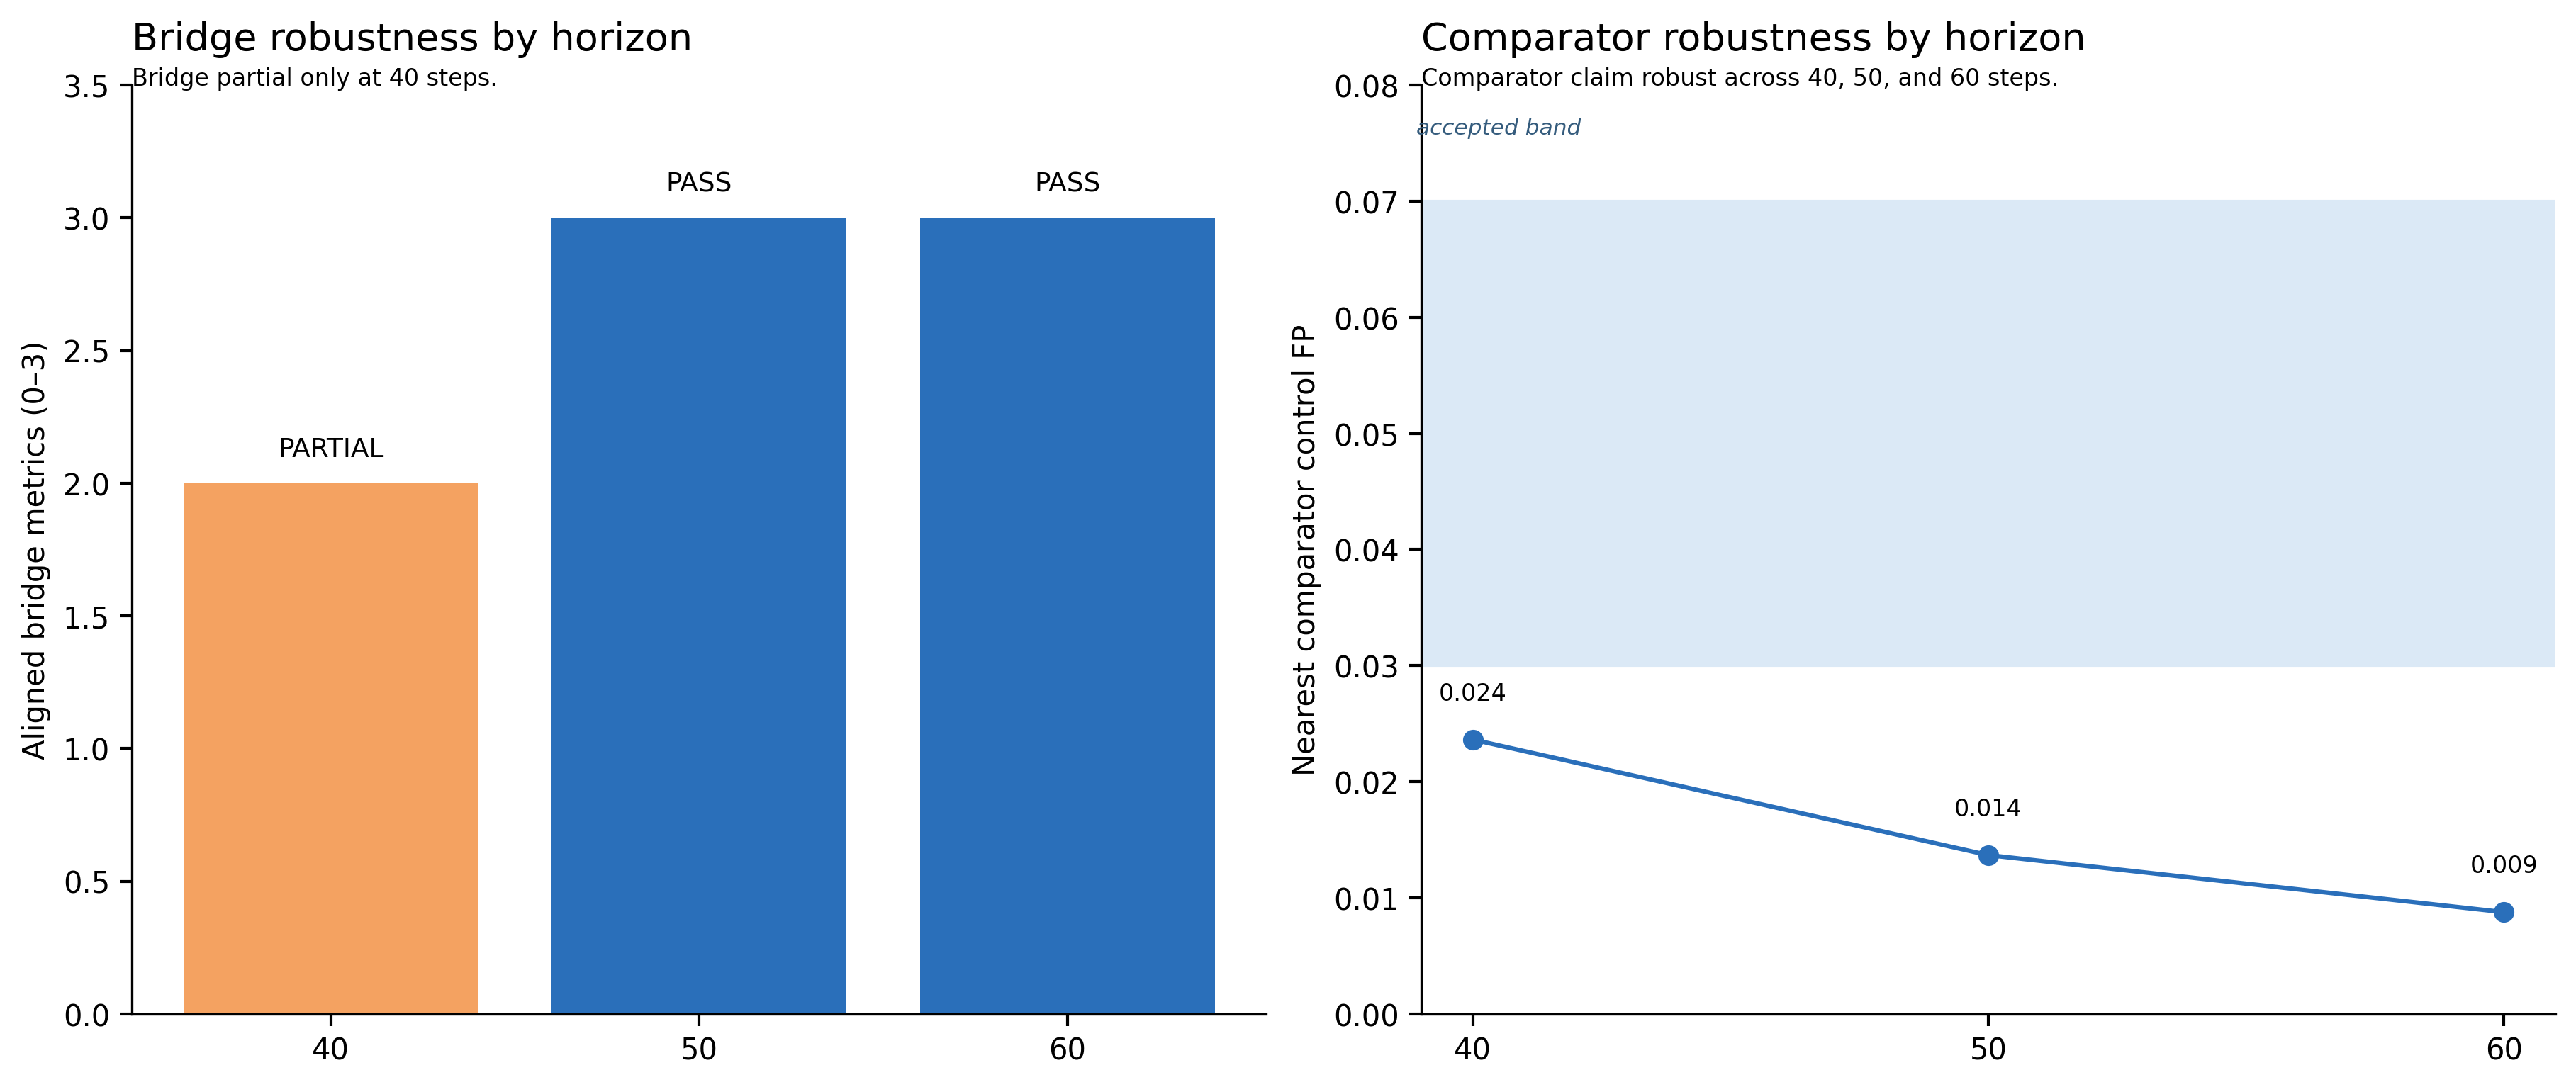
\includegraphics[keepaspectratio]{assets/fig3_recommender_horizon_sensitivity.png}}

\textbf{Figure 2. Recommender robustness by adjacent horizon
sensitivity.} The bridge criterion is satisfied at 50 and 60 steps and
only partially satisfied at 40 steps, indicating bounded horizon
sensitivity rather than failure of the empirical program. The comparator
claim is robust across all three horizons: no tested comparator
configuration is accepted at 40, 50, or 60 steps. Results are based on
offline deterministic replay rather than deployed-system feedback.

\subsubsection{Public market event
family}\label{public-market-event-family}

Public markets provide a stringent test because they combine exogenous
shocks, endogenous amplification (Brunnermeier \& Pedersen, 2009),
volatility-linked stress indicators such as the VIX (Whaley, 2009; ESRB
Advisory Scientific Committee, 2019), heterogeneous liquidity structure,
and a substantial comparator literature. We therefore assembled a
reproducible public market event family centered on the February 2018
Volmageddon dislocation (Augustin et al., 2021) and the March 2020 COVID
market-wide circuit-breaker cluster (NYSE Market-Wide Circuit Breaker
Working Group, 2020), together with hard negative controls. The purpose
was not to present markets as a universal separator domain, but to ask
whether a formally specified recursive warning criterion survives
externally auditable benchmark construction in a domain with strong
prior comparators and obvious confounds.

In this branch, the critical distinction is between narrative motivation
and frozen benchmark evaluation. Narrative examples such as the 2010
Flash Crash (CFTC and SEC Staff, 2010) motivate the broader problem of
recursive dislocation, but the quantitative claims reported here are
anchored to the frozen canonical markets benchmark and its comparator
contract. That benchmark is the relevant object for comparator
availability, equal-false-positive reachability, and robustness.

\subsubsection{Comparator calibration on the canonical markets
benchmark}\label{comparator-calibration-on-the-canonical-markets-benchmark}

To test whether the markets result depended on a narrow comparator set,
we evaluated a broader comparator suite on the canonical segmented
markets benchmark, volmageddon\_covid\_public\_v2, constructed from a
single canonical source configuration and a rule in which one underlying
market segment constituted one comparator unit. This yielded 38 control
units and 16 event units, so the prespecified equal-false-positive
acceptance band, FP ∈ {[}0.03, 0.07{]}, was reachable on this benchmark
with grid step 1/38 = 0.026316. Fast comparator families comprised
variance EWS and lag-1 autocorrelation (AC1) (Dakos et al., 2012),
CUSUM, and Page-Hinkley; slow families comprised matrix profile and
permutation entropy. All families were evaluated under the same locked
equal-false-positive contract with predeclared parameter grids, followed
by full-grid expansion of the slow families on the frozen canonical
benchmark.

No tested fast or slow comparator configuration achieved the acceptance
band on the canonical markets benchmark. The nearest nontrivial
comparator remained AC1: configuration ac1\_ews\_\_632f23b2 alarmed on
5/38 control units (FP = 0.131579) and 1/16 event units, leaving it
0.061579 above the admissible band. Full-grid slow-family evaluation did
not rescue the comparator branch. The numerically nearest slow
configurations were tied across matrix profile and permutation entropy,
but both were trivial-silent, producing 0/38 control alarms and 0/16
event alarms. Among slow families, the best nontrivial configuration
came from permutation entropy (permutation\_entropy\_\_259c1b96), which
alarmed on 14/38 control units (FP = 0.368421) and 4/16 event units,
remaining 0.298421 above band. Thus, under a reachable and locked
equal-false-positive criterion, no tested comparator configuration
admitted an acceptable operating point on the canonical markets
benchmark.

\pandocbounded{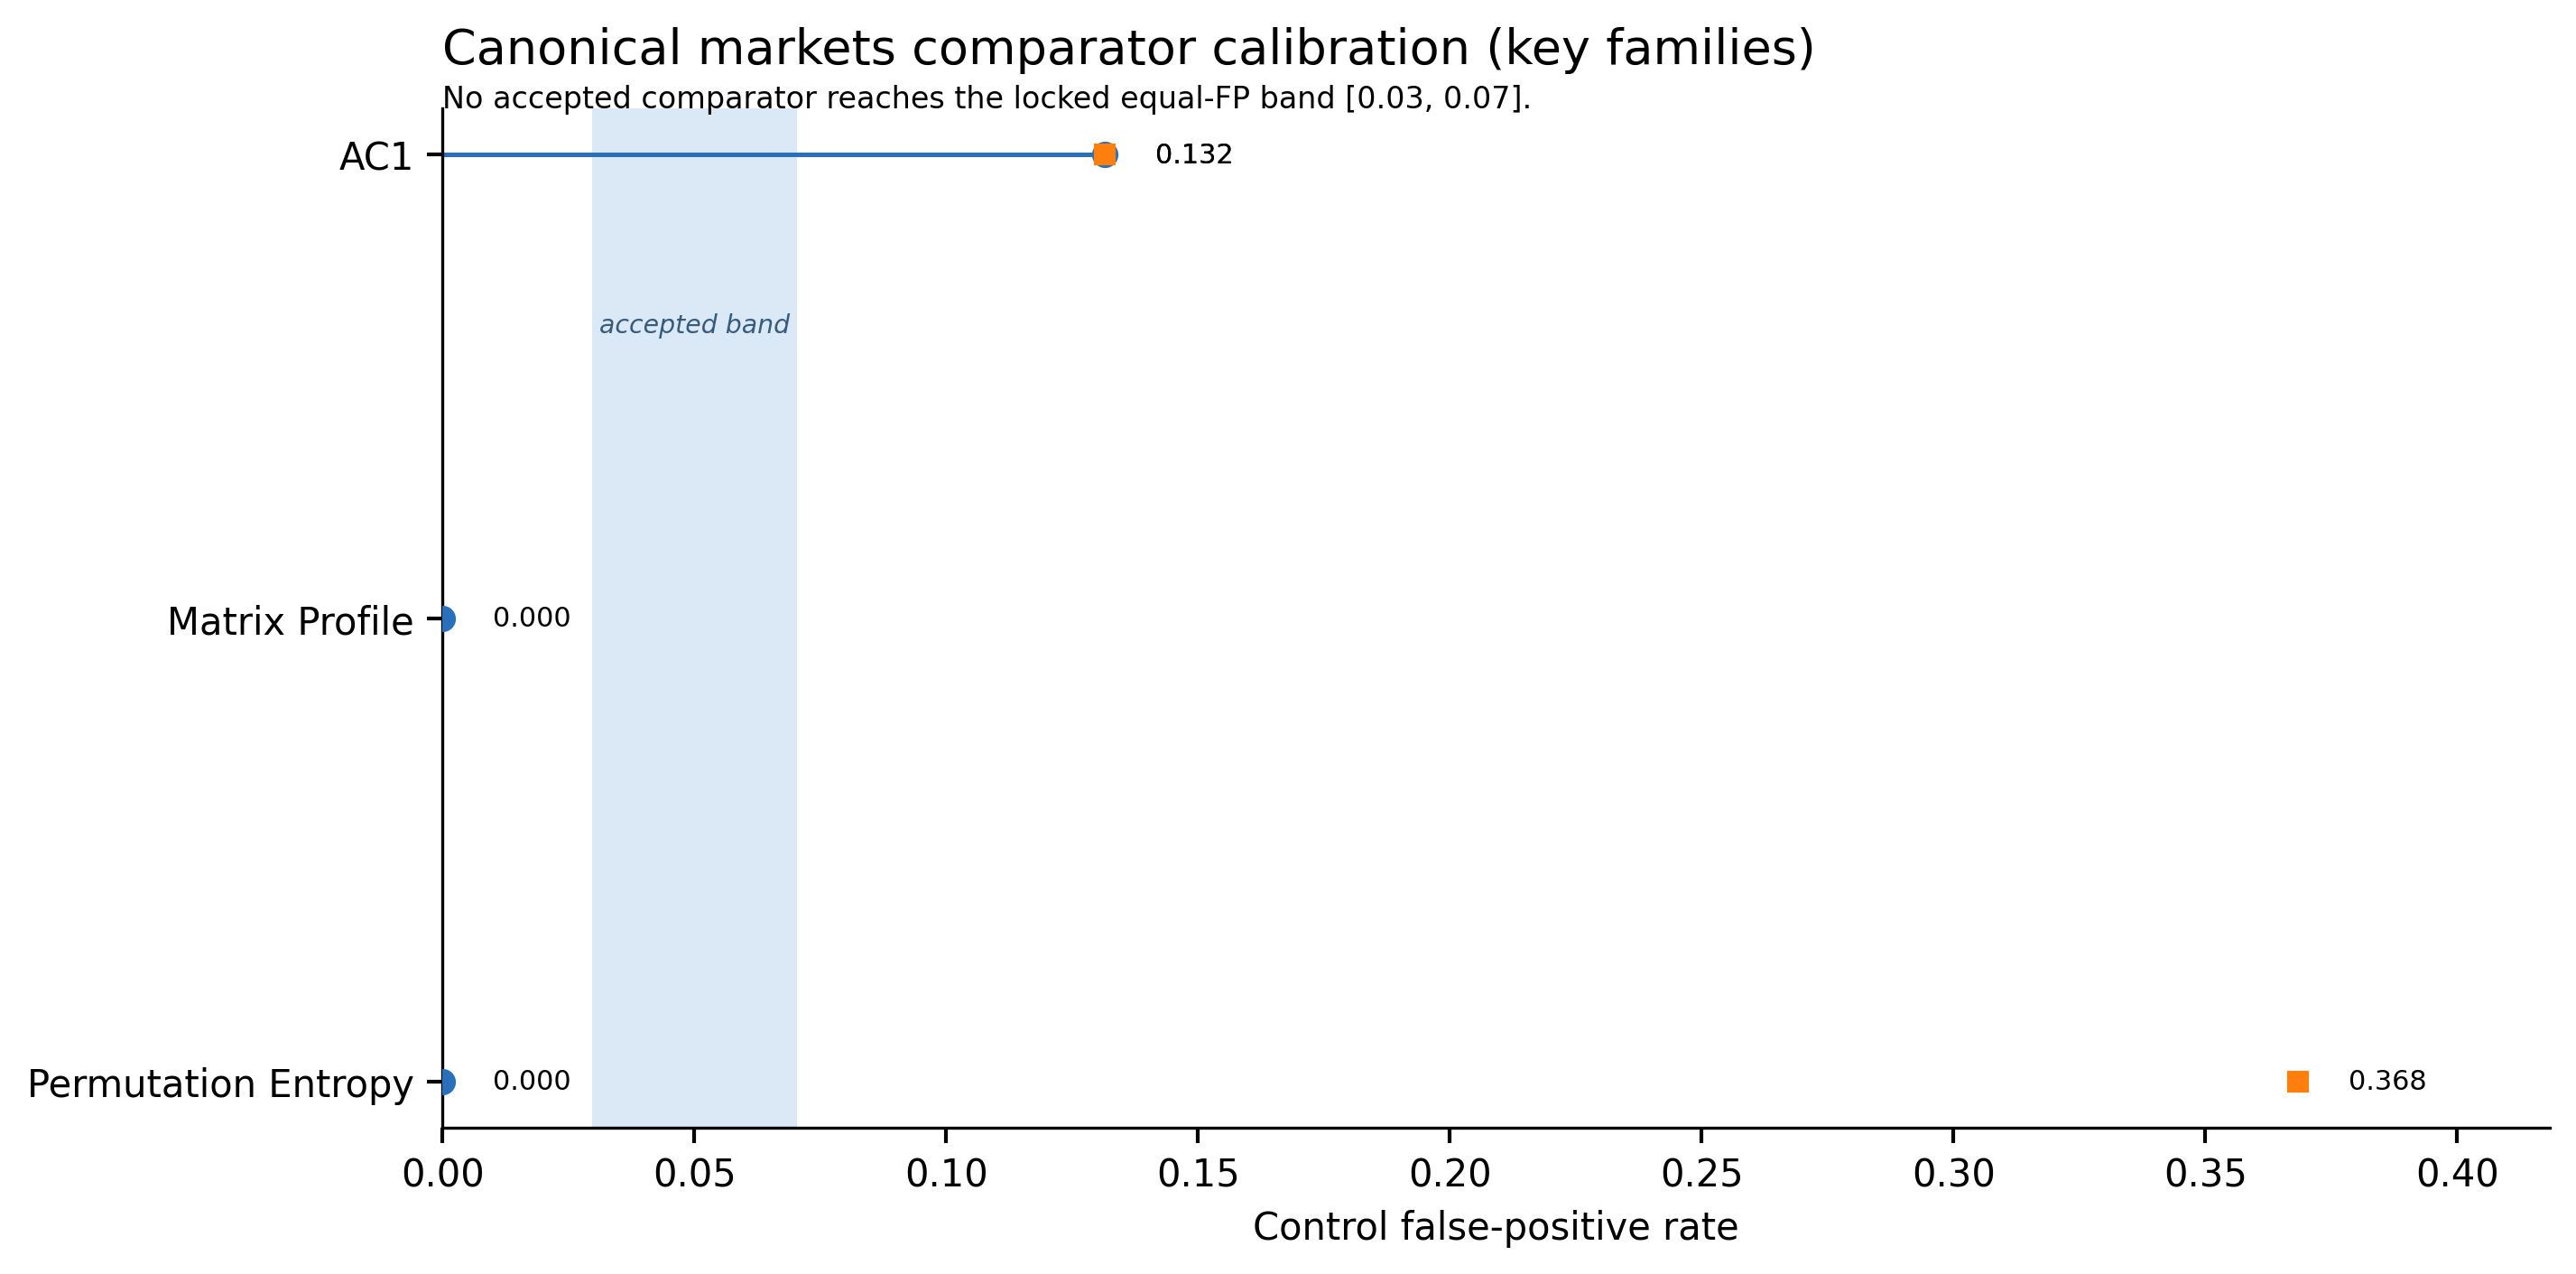
\includegraphics[keepaspectratio]{assets/fig1_markets_canonical_comparator_band.png}}

\textbf{Figure 3. Comparator calibration on the canonical segmented
markets benchmark.} No tested fast or slow comparator configuration
reaches the locked equal-false-positive band {[}0.03, 0.07{]}. The
nearest nontrivial comparator is AC1 at FP = 0.131579 (5/38 control
alarm units), while the numerically nearest slow configurations are
trivial-silent and the best nontrivial slow family, permutation entropy,
remains materially above band.

\subsubsection{Fast-family robustness under canonical and relaxed band
specifications}\label{fast-family-robustness-under-canonical-and-relaxed-band-specifications}

The comparator conclusion in markets admits a narrower and more precise
robustness statement. Under the prespecified equal-false-positive band
{[}0.03, 0.07{]}, no tested fast-family comparator configuration was
accepted on the canonical 120-minute segmented markets benchmark or on
60-minute and 180-minute segmentation sensitivity variants. In all three
cases, the nearest fast family remained AC1; the nearest false-positive
rate was 0.1316 for the canonical 120-minute units, 0.0800 for the
60-minute units, and 0.1304 for the 180-minute units. Thus, fast-family
non-acceptance was robust across tested segmentations at the locked
canonical specification.

By contrast, post-processing band-sensitivity analysis showed that
widening the acceptable interval to {[}0.02, 0.08{]} or {[}0.04, 0.08{]}
admitted the 60-minute AC1 configuration, whereas the canonical
120-minute and 180-minute segmentations remained non-accepted. We
therefore distinguish canonical robustness from relaxed-band sensitivity
and do not claim full invariance to post hoc band relaxation. The result
that carries manuscript weight is the stronger one: at the prespecified
canonical band, no fast-family comparator is accepted at 60-, 120-, or
180-minute segmentation.

\subsubsection{Controls, falsification boundary, and bounded
exceptions}\label{controls-falsification-boundary-and-bounded-exceptions}

The bridge criterion is explicitly falsifiable. It would be weakened if
externally defined collapse events occurred without prior increase in G
and p and decrease in δ; if comparator configurations detected the same
events under matched false-positive constraints without exhibiting this
triad; if the (G, p, δ) pattern appeared frequently in control periods
without progression toward externally defined collapse; or if
alternative reasonable operationalizations of amplification, recursive
persistence, and diversity contraction failed to agree directionally
with the present measurements. At the benchmark level, the empirical
program would be invalidated if any comparator configuration achieved an
accepted operating point on the canonical benchmark under the same
equal-false-positive contract.

The markets branch also contains a bounded near-miss rather than a
universal separator. Binary and topological diagnostics did not separate
Volmageddon from vol-heavy hard negatives. The strongest remaining
signal instead appeared in continuous witness quality, with the clearest
confirmation in corroborating configuration cfg\_002053, particularly
against volmageddon\_control\_2018\_02\_08. We therefore treat this
residual as a bounded exception that sharpens the empirical
interpretation rather than as a contradiction of the broader result.
Across the retained domains, we do not observe either falsifying
condition.

\subsubsection{Third-domain corroboration: LLM training-loop collapse
(secondary
analysis)}\label{third-domain-corroboration-llm-training-loop-collapse-secondary-analysis}

\pandocbounded{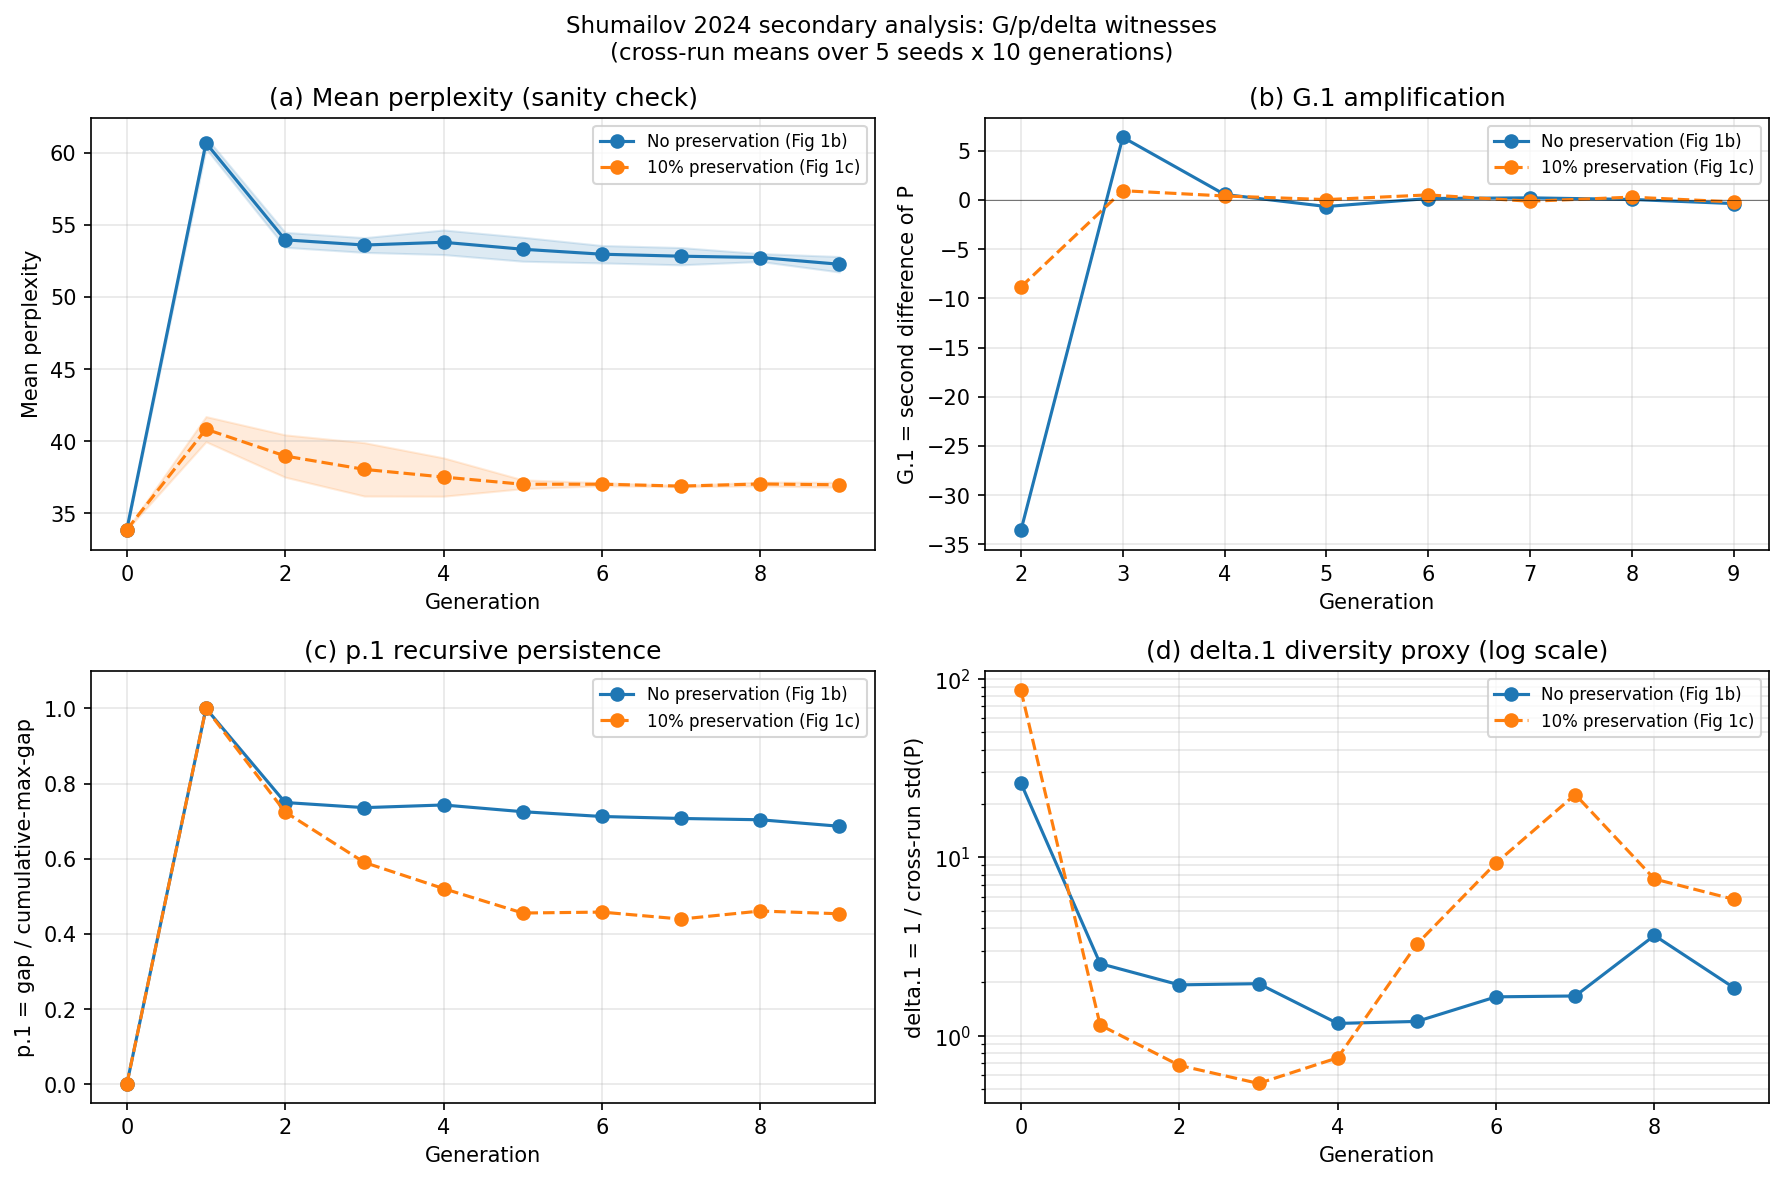
\includegraphics[keepaspectratio]{assets/fig4_shumailov_witness_triad.png}}

\textbf{Figure 4.} G/p/δ witnesses across 10 generations of recursive
LLM fine-tuning, secondary analysis on data digitized from Shumailov et
al.~(2024) Figure 1b/1c right panels. Lines show cross-run means over 5
random-seed runs. (a) Mean perplexity sanity check with ±1σ envelope.
(b) G.1 amplification (second difference of mean perplexity per run);
large negative deflection at generation 2 marks the phase-transition
signature. (c) p.1 recursive persistence (gap-to-cumulative-max ratio);
jumps to 1 at collapse onset and stays elevated. (d) δ.1 diversity proxy
(inverse cross-run perplexity standard deviation, log scale); declines
sharply at onset in both regimes. Two regimes shown: no preservation
(blue, Fig 1b) and 10\% real-data preservation (orange, Fig 1c).

Recursive language-model training exhibits the same closed-loop topology
as the markets and recommender domains: model outputs become inputs to
the next generation's training, creating conditions for
self-amplification and diversity contraction. Shumailov et al.~(2024)
demonstrated this empirically, showing that perplexity on held-out text
rises sharply within one generation of fine-tuning on synthetic data and
stabilizes at an elevated plateau, with magnitude depending on whether
real data is preserved across generations. We use this third recursive
domain as a corroboration test for the G/p/δ witness triad, conducted as
secondary analysis rather than as a matched-FP benchmark.

We digitized mean perplexity values from Figure 1b/1c right panels of
Shumailov et al.~(five random-seed runs across ten recursive
generations, in two preservation regimes: no preservation and 10\%
preservation). Each witness was computed from per-generation perplexity
data: G.1 as the second difference of mean perplexity per run, p.1 as
the ratio of the current perplexity-gap to the per-run
cumulative-maximum gap, and δ.1 as the inverse of cross-run perplexity
standard deviation at each generation. Generation 0 (the Real wikitext2
baseline) is the control window; generations 1 through 9 are the event
window.

All three witnesses move in the predicted direction across the collapse
transition in both regimes (Figure 4). G.1 shows a sharp
phase-transition signature: \textbar G\textbar{} at generation 2 is
22.6× the steady-state mean in the no-preservation regime and 16.7× in
the 10\%-preservation regime. p.1 jumps from 0 at baseline to
approximately 1 at generation 1 and never relaxes below 0.36 in either
regime. δ.1 declines sharply at onset (control/event ratio 13.3× and
15.0×). The framework generates three graded predictions, all of which
the data also support: G.1 transition magnitude scales with collapse
severity (3.8× larger without preservation); p.1 plateau height encodes
the regime (0.75 versus 0.45); δ.1 partially recovers in the
10\%-preservation regime as random seeds re-converge to a stable
collapsed attractor.

We do not claim a third benchmark. Values are digitized from published
figures rather than provided by the original authors, the δ.1
operationalization captures inter-seed convergence rather than the
within-model distributional diversity that the paper's Theorem 3.1
directly addresses, and no comparator-acceptance evaluation under a
matched false-positive contract was conducted for this domain. The full
benchmark - including experimental pipeline reconstruction at scale and
matched-FP evaluation - is deferred to follow-up work.

\subsubsection{Discussion}\label{discussion}

The scientific claim of the paper is deliberately minimal. First,
collapse in recursive systems can be rendered computable through a
formally specified observable predicate with an explicit claim boundary.
Second, under equal-false-positive fairness, tested standard comparator
configurations did not recover the same admissible operating behavior on
canonical benchmarks. The significance of the paper lies in the
conjunction of those two claims: a formal obstruction motivates a
conditional measurable pre-collapse signature, and that signature
survives fair benchmarking against a broad comparator suite. Unlike
threshold-tuned detectors, the empirical program is explicitly
falsifiable under a fixed equal-false-positive contract.

The markets branch is especially informative because it is both strong
and bounded. It is strong in the sense that the canonical segmented
benchmark is externally grounded, the acceptance band is reachable, the
comparator suite is broad, and no tested fast or slow configuration
admits an accepted operating point. It is bounded in the sense that the
60-minute fast-family branch becomes admissible only under widened post
hoc bands, and the Volmageddon residual is not presented as a universal
separator. That boundedness is scientifically useful. It marks the
difference between a detector paper that optimizes narrative smoothness
and a theory-led manuscript that preserves the structure of its own
exceptions.

The recommender branch provides a second flagship empirical benchmark,
drawn from offline deterministic replay of MovieLens-25M user
trajectories rather than from a deployed recommender system. On the
canonical 50-step MovieLens recursive frontier benchmark, the bridge
criterion was satisfied and no tested fast or slow comparator
configuration admitted an accepted operating point under the locked
equal-false-positive rule. Adjacent-horizon sensitivity preserves the
comparator result at 40 and 60 steps, while the bridge criterion is
satisfied at 50 and 60 and only partially satisfied at 40. The
recommender evidence therefore supports a corroborating second flagship
benchmark with bounded bridge sensitivity under adjacent horizon
shortening rather than a claim of unqualified invariance.

The third domain - recursive LLM training-loop collapse (Shumailov et
al., 2024) - was evaluated as secondary analysis rather than as a
matched-FP benchmark. All three witnesses moved in the predicted
direction across the collapse transition in both preservation regimes,
with three graded predictions also visible: transition magnitude scales
with collapse severity, persistence plateau height encodes the
preservation regime, and diversity partially recovers in the
10\%-preservation regime as seeds re-converge to a stable collapsed
attractor. The third-domain evidence therefore corroborates the witness
triad's directional structure beyond the two flagship benchmarks, while
matched-FP comparator evaluation in this domain is deferred to follow-up
work.

Several limitations remain. Witness construction is still
domain-adapted. Comparator scope could expand further. And the bridge
criterion, although explicit and falsifiable here, remains empirical
rather than an identification result. The next scientific step is
therefore not rhetorical expansion but stress-testing: additional
domains under full matched-FP comparator evaluation, external
replication, intervention logic, and broader comparator classes. The
present results support a precise claim: a formally specified recursive
collapse obstruction defines an explicit route to a measurable
pre-collapse footprint that can be evaluated under a fair alert-budget
benchmark, and across the canonical public markets and recommender
benchmarks no tested standard comparator configuration achieves an
accepted operating point under that contract.

\subsubsection{Materials and Methods
(brief)}\label{materials-and-methods-brief}

The paper combines a Lean-formalized minimal obstruction (de Moura \&
Ullrich, 2021; The mathlib Community, 2020) with empirical witness
construction over gain, recursive persistence, and diversity. The public
Lean keeper surface includes \texttt{no\_progress\_cycle\_public},
\texttt{no\_progress\_kcycle\_public},
\texttt{collapse\_via\_progresscycle\_public}, \texttt{TelemetryState},
\texttt{telemetryμ}, \texttt{telemetry\_bridge\_obstruction\_public},
and \texttt{no\_telemetry\_forbidden\_cycle\_public}. Empirical
evaluation is performed under a locked equal-false-positive contract, so
detector families are compared at the same alert budget rather than at
arbitrary thresholds. Bridge satisfaction is operationally defined as
follows: under the prespecified pre-collapse window, event-unit
summaries of G are higher than control-unit summaries, p maintains its
non-relaxation property, and event-unit summaries of δ are lower than
control-unit summaries; bridge non-satisfaction is defined as failure of
any of these conditions. In markets, the expanded comparator suite
included variance EWS, AC1, CUSUM, Page-Hinkley, matrix profile, and
permutation entropy, all evaluated under the same locked
equal-false-positive contract on the canonical segmented benchmark and
its adjacent robustness variants. In recommenders, a public
MovieLens-25M recursive frontier benchmark was constructed from one
episode per user under a deterministic item-item replay engine, with
collapse defined by failure to recover held-out positive frontier items
under frozen benchmark rules. Across both domains, the witness triplet
(G, p, δ) was evaluated as an empirical instantiation of the formal
collapse obstruction under the assumptions stated in the bridge
criterion and Supplementary Materials. Full benchmark construction,
parameter grids, robustness packets, bridge assumptions, falsification
conditions, and availability outcomes are reported in the Supplementary
Materials.

\textbf{Markets benchmark construction.} The canonical segmented markets
benchmark \texttt{volmageddon\_covid\_public\_v2} (canonical Loopzero
configuration \texttt{cfg\_001339}) was constructed from a curated set
of intraday packet ingredients drawn from minute-bar data for six
US-listed instruments --- SPY, QQQ, IWM, VXX, UVXY, and SVXY ---
covering the Volmageddon dislocation (February 2018; Augustin et al.,
2021) and the March 2020 COVID market-wide circuit-breaker cluster (NYSE
MWCB Working Group, 2020). Each canonical packet contains preprocessed
Loopzero telemetry (G, p, δ) for one underlying time series;
non-canonical configurations were excluded to avoid duplicated session
units. Each packet was sliced into 120-minute time-window segments
(minimum 60 retained minute-bars per segment), and each (slice ×
segment) pair became one comparator unit. Event/control assignment was
made by membership of the slice identifier in a prespecified list of
canonical event identifiers (e.g., \texttt{volmageddon\_2018\_xiv},
\texttt{covid\_mwcb\_2020\_03\_18}), with hard negative controls drawn
from non-event slices over the same instrument universe. Under this
construction, 38 control units and 16 event units were retained,
yielding an FP grid step of 1/38 = 0.026316. Calibration semantics are
full-benchmark with per-unit rolling-quantile thresholds and no held-out
partition. Because each segment is treated as an independent comparator
unit during calibration, intra-event correlation under shared
market-wide stress is acknowledged as a dependence limitation and is
identified as a target for follow-up sensitivity analysis.

\textbf{Recommender benchmark construction.} The canonical recursive
recommender benchmark
\texttt{movielens25m\_recursive\_frontier\_public\_v1} was constructed
from the public MovieLens-25M dataset
(https://grouplens.org/datasets/movielens/25m/). Per-user trajectories
were sorted chronologically and reduced to one episode per user. Each
episode was replayed under a deterministic item-item
collaborative-filtering engine with a warm-start prefix and a held-out
positive frontier; collapse was defined as failure to recover held-out
positive-frontier items under frozen benchmark rules. The canonical
horizon was 50 recursive update steps; adjacent horizons of 40 and 60
steps were tested for bridge-sensitivity robustness. Under the canonical
50-step construction, 40,339 user-level units satisfied inclusion
criteria, of which 35,584 were event units (collapse occurred within the
canonical horizon) and 4,755 were control units (collapse did not occur
within the canonical horizon), yielding an FP grid step of 1/4755 ≈
0.0002103. Comparator families were evaluated against a derived per-user
benchmark series, \texttt{miss\_run\_fraction}, capturing recursive
frontier-miss runs over the canonical horizon. Each user is treated as
an independent unit in calibration. Full parameter specification ---
including the positive-rating threshold, frontier size, warm-start
prefix length, item-item engine configuration, and leakage-prevention
rules --- is recorded in the canonical manuscript freeze state
(\texttt{movielens25m\_recursive\_frontier\_public\_v1\_\_manuscript\_freeze\_state.json}),
with construction details documented in the Supplementary Materials.

\textbf{Artifact availability.} The Lean keeper surface listed above is
publicly archived at
https://github.com/davidmullett/loopzero-paper-public (commit
\texttt{3b8c01c6884b23be0f5b9567d3fe965e7f682c23}) and is reproducible
under Lean v4.30.0-rc2 with Mathlib at commit
\texttt{3ba1ec58ec69cd649b9e5c61485a98d1dd37a00f}. The build runs
cleanly under \texttt{lake\ build}. An axiom audit verifies that the
three obstruction theorems (\texttt{no\_progress\_cycle\_public},
\texttt{no\_progress\_kcycle\_public},
\texttt{collapse\_via\_progresscycle\_public}) compile without any axiom
dependencies, while the two telemetry-bridge theorems
(\texttt{telemetry\_bridge\_obstruction\_public},
\texttt{no\_telemetry\_forbidden\_cycle\_public}) depend only on the
standard Mathlib trusted base (\texttt{propext},
\texttt{Classical.choice}, \texttt{Quot.sound}). No non-standard axioms
appear in the keeper surface.

\begin{center}\rule{0.5\linewidth}{0.5pt}\end{center}

\subsection{Figure and Table Legends}\label{figure-and-table-legends}

\textbf{Supplementary Figure S1. Fast-family segmentation and band
sensitivity on the canonical markets benchmark.} No fast-family
comparator was accepted at 60-, 120-, or 180-minute segmentation under
the prespecified equal-false-positive band {[}0.03, 0.07{]}. Under
widened post-processing bands with upper cutoff 0.08, acceptance
appeared only for the 60-minute AC1 configuration; the canonical
120-minute and 180-minute segmentations remained non-accepted across all
tested bands.

\begin{center}\rule{0.5\linewidth}{0.5pt}\end{center}

\subsection{References}\label{references}

Augustin, P., Chen, C. and Van den Bergen, H. (2021). Volmageddon and
the failure of short volatility products. \emph{Financial Analysts
Journal}. https://doi.org/10.1080/0015198x.2021.1913040

Boettiger, C. and Hastings, A. (2012a). Early warning signals and the
prosecutor's fallacy. \emph{Proc. Royal Society B}.
https://doi.org/10.1098/rspb.2012.2085

Boettiger, C. and Hastings, A. (2012b). Quantifying limits to detection
of early warning for critical transitions. \emph{Journal of the Royal
Society Interface}. https://doi.org/10.1098/rsif.2012.0125

Brunnermeier, M.K. and Pedersen, L.H. (2009). Market liquidity and
funding liquidity. \emph{Review of Financial Studies}.
https://doi.org/10.1093/rfs/hhn098

Buldyrev, S.V., Parshani, R., Paul, G., Stanley, H.E. and Havlin, S.
(2010). Catastrophic cascade of failures in interdependent networks.
\emph{Nature}. https://doi.org/10.1038/nature08932

Carpenter, S.R., Cole, J.J., Pace, M.L., Batt, R., Brock, W.A., Cline,
T. et al.~(2011). Early warnings of regime shifts: A whole-ecosystem
experiment. \emph{Science}. https://doi.org/10.1126/science.1203672

CFTC and SEC Staff (2010). Findings Regarding the Market Events of May
6, 2010. Report, SEC / CFTC.
https://www.sec.gov/news/studies/2010/marketevents-report.pdf

Chaney, A.J.B., Stewart, B.M. and Engelhardt, B.E. (2018). How
algorithmic confounding in recommendation systems increases homogeneity
and decreases utility. \emph{ACM RecSys}.
https://doi.org/10.1145/3240323.3240370

Dakos, V., Carpenter, S.R., Brock, W.A., Ellison, A.M., Guttal, V.,
Ives, A.R. et al.~(2012). Methods for detecting early warnings of
critical transitions in time series illustrated using simulated
ecological data. \emph{PLOS ONE}.
https://doi.org/10.1371/journal.pone.0041010

de Moura, L. and Ullrich, S. (2021). The Lean 4 Theorem Prover and
Programming Language. \emph{CADE-28}.
https://doi.org/10.1007/978-3-030-79876-5\_37

Diks, C., Hommes, C. and Wang, J. (2019). Systematically false positives
in early warning signal analysis. \emph{PLOS ONE}.
https://doi.org/10.1371/journal.pone.0211072

ESRB Advisory Scientific Committee (2019). Can ETFs Contribute to
Systemic Risk? Report, ESRB.
https://www.esrb.europa.eu/pub/pdf/asc/esrb.asc190617\_9\_canetfscontributesystemicrisk\textasciitilde983ea11870.en.pdf

Fleder, D. and Hosanagar, K. (2009). Blockbuster culture's next rise or
fall: The impact of recommender systems on sales diversity.
\emph{Management Science}. https://doi.org/10.1287/mnsc.1080.0974

Gao, J., Barzel, B. and Barabasi, A.-L. (2016). Universal resilience
patterns in complex networks. \emph{Nature}.
https://doi.org/10.1038/nature16948

Hanley, J.A. and McNeil, B.J. (1982). The meaning and use of the area
under a receiver operating characteristic (ROC) curve. \emph{Radiology}.
https://doi.org/10.1148/radiology.143.1.7063747

Holling, C.S. (1973). Resilience and stability of ecological systems.
\emph{Annual Review of Ecology and Systematics}.
https://doi.org/10.1146/annurev.es.04.110173.000245

Jiang, R., Chiappa, S., Lattimore, T., Gyorgy, A. and Kohli, P. (2019).
Degenerate feedback loops in recommender systems. \emph{AIES/ACM}.
https://doi.org/10.1145/3306618.3314288

Mansoury, M., Abdollahpouri, H., Pechenizkiy, M., Mobasher, B. and
Burke, R. (2020). Feedback loop and bias amplification in recommender
systems. \emph{CIKM}. https://doi.org/10.1145/3340531.3412152

NYSE Market-Wide Circuit Breaker (MWCB) Working Group (2020). Report of
the Market-Wide Circuit Breaker (MWCB) Working Group. Report, NYSE /
SEC.
https://www.nyse.com/publicdocs/nyse/markets/nyse/Report\_of\_the\_Market-Wide\_Circuit\_Breaker\_Working\_Group.pdf

Scheffer, M., Carpenter, S., Foley, J.A., Folke, C. and Walker, B.
(2001). Catastrophic shifts in ecosystems. \emph{Nature}.
https://doi.org/10.1038/35098000

Scheffer, M., Bascompte, J., Brock, W.A., Brovkin, V., Carpenter, S.R.,
Dakos, V. et al.~(2009). Early-warning signals for critical transitions.
\emph{Nature}. https://doi.org/10.1038/nature08227

Scheffer, M., Carpenter, S.R., Lenton, T.M., Bascompte, J., Brock, W.,
Dakos, V. et al.~(2012). Anticipating critical transitions.
\emph{Science}. https://doi.org/10.1126/science.1225244

Shumailov, I., Shumaylov, Z., Zhao, Y., Papernot, N., Anderson, R. and
Gal, Y. (2024). AI models collapse when trained on recursively generated
data. \emph{Nature}. https://doi.org/10.1038/s41586-024-07566-y

The mathlib Community (2020). The Lean mathematical library. \emph{CPP
(ACM SIGPLAN)}. https://doi.org/10.1145/3372885.3373824

Walker, B., Holling, C.S., Carpenter, S.R. and Kinzig, A. (2004).
Resilience, adaptability and transformability in social-ecological
systems. \emph{Ecology and Society}.
https://doi.org/10.5751/ES-00650-090205

Whaley, R.E. (2009). Understanding the VIX. \emph{Journal of Portfolio
Management}. https://doi.org/10.3905/jpm.2009.35.3.098

\end{document}
